\documentclass[tikz,border=8pt]{standalone}
\usepackage[T1]{fontenc}
\usepackage{tikz}
\usetikzlibrary{arrows.meta,positioning,fit,backgrounds,calc}
\definecolor{blue}{RGB}{32,94,180}
\definecolor{green}{RGB}{43,150,136}
\definecolor{purple}{RGB}{105,98,178}
\definecolor{gold}{RGB}{190,132,45}
\definecolor{orange}{RGB}{194,115,45}
\definecolor{grayline}{RGB}{91,99,112}
\definecolor{softgray}{RGB}{247,249,252}
\definecolor{textgray}{RGB}{35,42,54}
\tikzset{
  nodebox/.style={draw=#1, fill=#1!8, rounded corners=3pt, thick, align=center,
    minimum width=34mm, minimum height=11mm, text=textgray, font=\sffamily\small},
  widebox/.style={draw=#1, fill=#1!8, rounded corners=3pt, thick, align=center,
    minimum width=43mm, minimum height=12mm, text=textgray, font=\sffamily\small},
  corebox/.style={draw=#1, fill=#1!8, rounded corners=4pt, very thick, align=center,
    minimum width=50mm, minimum height=18mm, text=textgray, font=\sffamily\small},
  databox/.style={draw=#1, fill=#1!8, rounded corners=4pt, very thick, align=center,
    minimum width=51mm, minimum height=17mm, text=textgray, font=\sffamily\small},
  packagebox/.style={draw=#1, fill=#1!4, rounded corners=4pt, thick, dashed,
    align=left, text=textgray, font=\sffamily\footnotesize,
    minimum width=62mm, minimum height=31mm, inner xsep=4mm, inner ysep=3mm},
  iconnode/.style={minimum width=28mm, minimum height=21mm, inner sep=0pt},
  lane/.style={font=\sffamily\bfseries\scriptsize, text=#1, align=left},
  note/.style={font=\sffamily\scriptsize, text=textgray, align=center},
  readnote/.style={font=\sffamily\scriptsize, text=textgray, align=center,
    fill=white, inner sep=1pt},
  arrow/.style={-{Latex[length=2.2mm]}, thick, draw=grayline},
  readarrow/.style={-{Latex[length=2.2mm]}, thick, draw=grayline!72, dashed},
  trustarrow/.style={-{Latex[length=2.2mm]}, very thick, draw=grayline}
}
\begin{document}
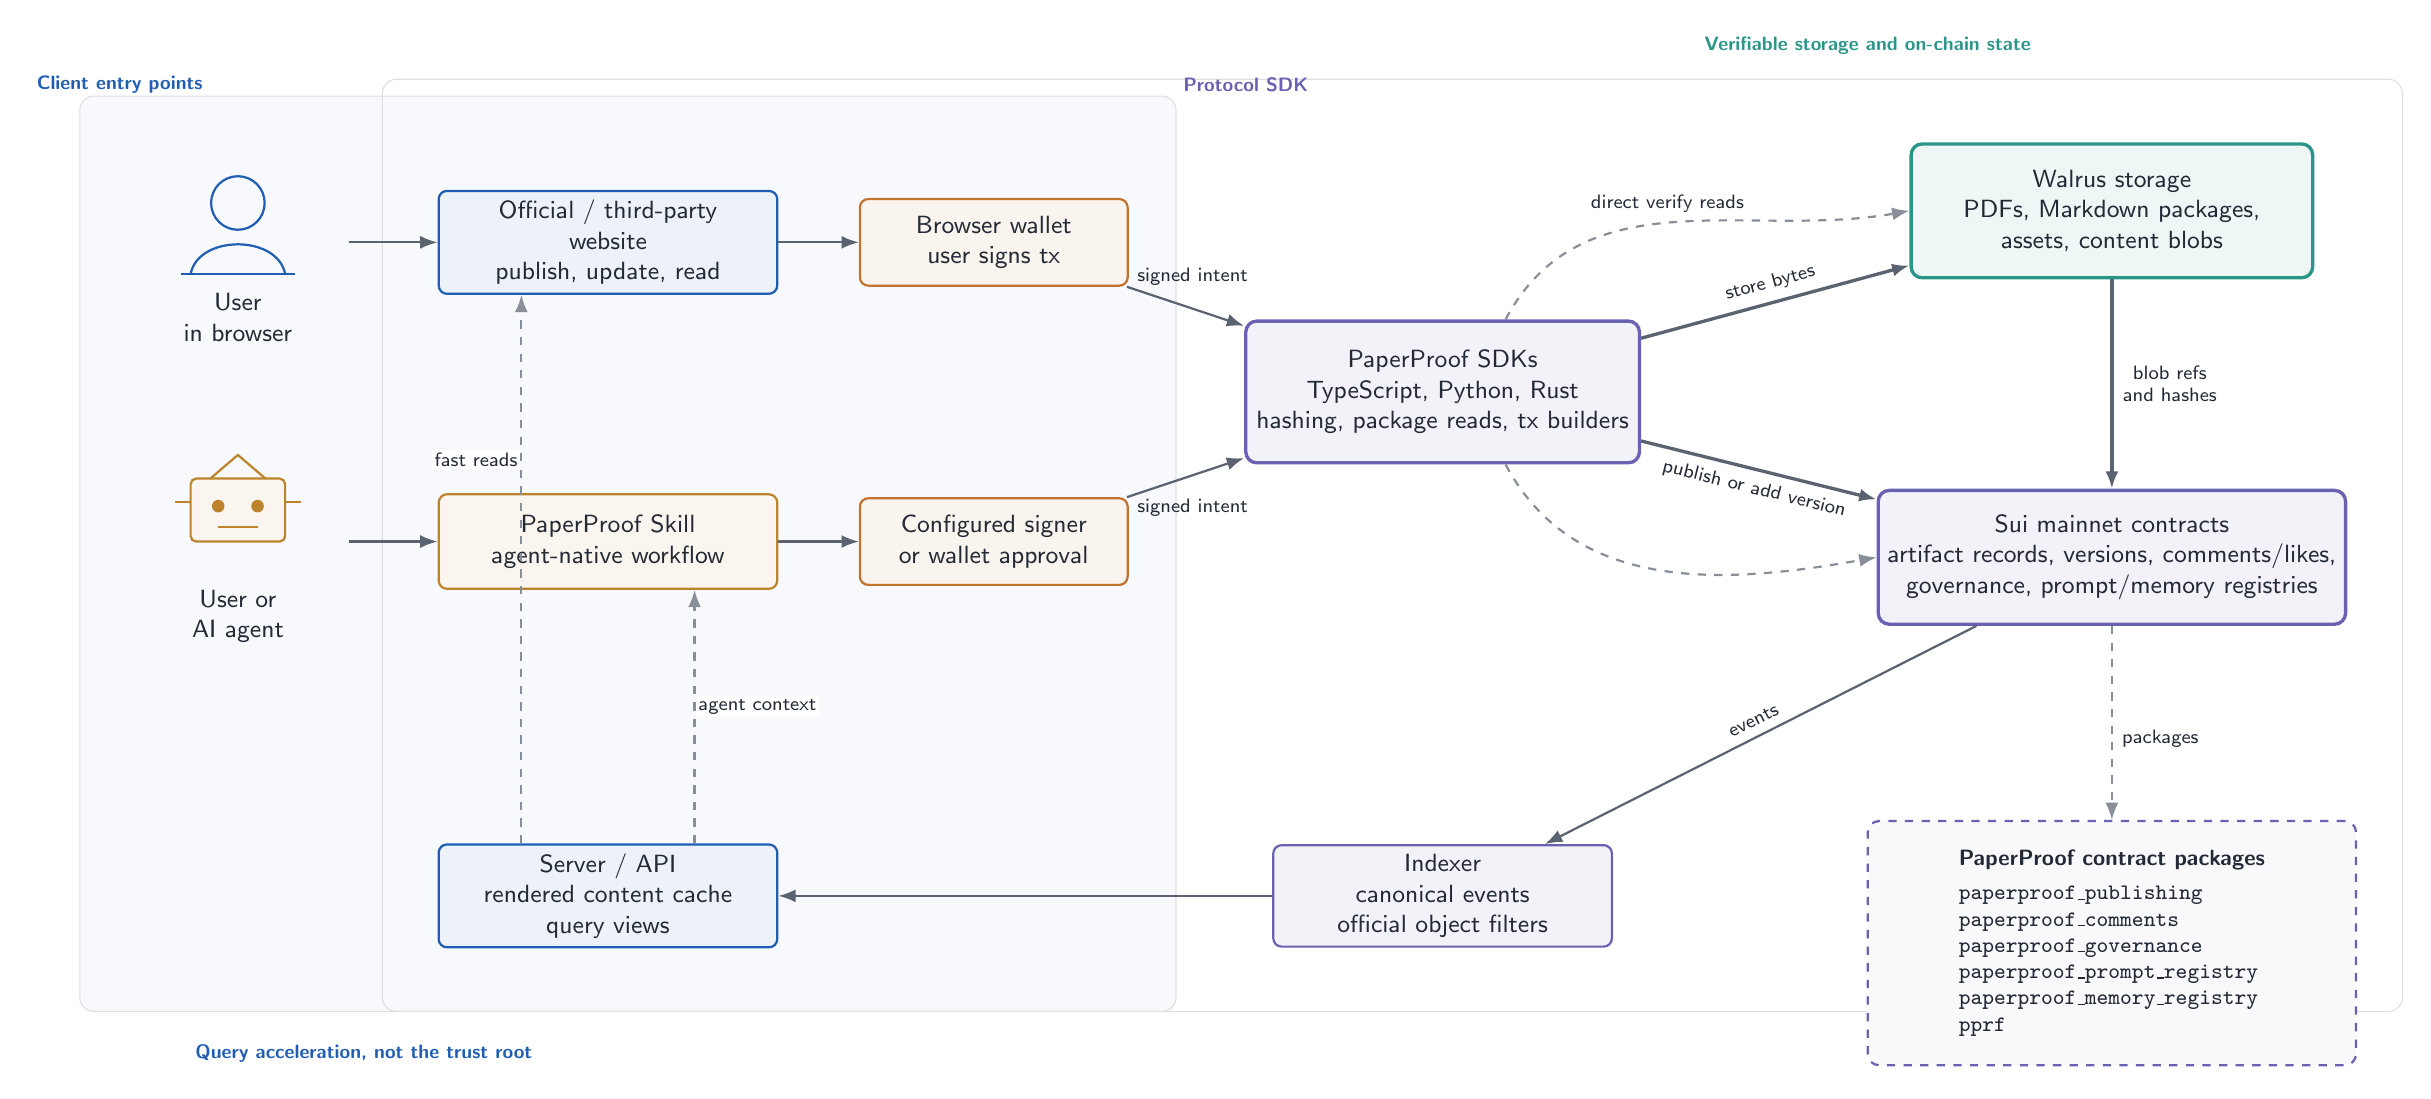
\begin{tikzpicture}[x=1mm,y=1mm]
  \node[iconnode] (browseruser) at (0,58) {};
  \draw[blue, thick] ($(browseruser.center)+(0,5)$) circle (3.4);
  \draw[blue, thick, rounded corners=4pt] ($(browseruser.center)+(-6,-4)$)
    .. controls ($(browseruser.center)+(-5,1)$) and ($(browseruser.center)+(5,1)$) ..
    ($(browseruser.center)+(6,-4)$);
  \draw[blue, thick] ($(browseruser.center)+(-7.2,-4)$) -- ($(browseruser.center)+(7.2,-4)$);
  \node[font=\sffamily\small, text=textgray, align=center] at ($(browseruser.center)+(0,-9.5)$) {User\\in browser};
  \node[widebox=blue] (website) at (47,58) {Official / third-party\\website\\publish, update, read};
  \node[nodebox=orange] (wallet) at (96,58) {Browser wallet\\user signs tx};

  \node[iconnode] (agentuser) at (0,20) {};
  \draw[gold, thick, rounded corners=2pt, fill=gold!8] ($(agentuser.center)+(-6,0)$) rectangle ($(agentuser.center)+(6,8)$);
  \draw[gold, thick] ($(agentuser.center)+(-3.5,8)$) -- ($(agentuser.center)+(0,11)$) -- ($(agentuser.center)+(3.5,8)$);
  \fill[gold] ($(agentuser.center)+(-2.5,4.5)$) circle (0.8);
  \fill[gold] ($(agentuser.center)+(2.5,4.5)$) circle (0.8);
  \draw[gold, thick] ($(agentuser.center)+(-2.5,1.8)$) -- ($(agentuser.center)+(2.5,1.8)$);
  \draw[gold, thick] ($(agentuser.center)+(-8,5)$) -- ($(agentuser.center)+(-6,5)$);
  \draw[gold, thick] ($(agentuser.center)+(6,5)$) -- ($(agentuser.center)+(8,5)$);
  \node[font=\sffamily\small, text=textgray, align=center] at ($(agentuser.center)+(0,-9.5)$) {User or\\AI agent};
  \node[widebox=gold] (skill) at (47,20) {PaperProof Skill\\agent-native workflow};
  \node[nodebox=orange] (signer) at (96,20) {Configured signer\\or wallet approval};

  \node[corebox=purple] (sdk) at (153,39) {PaperProof SDKs\\TypeScript, Python, Rust\\hashing, package reads, tx builders};

  \node[databox=green] (walrus) at (238,62) {Walrus storage\\PDFs, Markdown packages,\\assets, content blobs};
  \node[databox=purple] (sui) at (238,18) {Sui mainnet contracts\\artifact records, versions, comments/likes,\\governance, prompt/memory registries};

  \node[widebox=purple] (indexer) at (153,-25) {Indexer\\canonical events\\official object filters};
  \node[widebox=blue] (api) at (47,-25) {Server / API\\rendered content cache\\query views};
  \node[packagebox=purple] (packages) at (238,-31) {
    \textbf{PaperProof contract packages}\\[1mm]
    \texttt{paperproof\_publishing}\\
    \texttt{paperproof\_comments}\\
    \texttt{paperproof\_governance}\\
    \texttt{paperproof\_prompt\_registry}\\
    \texttt{paperproof\_memory\_registry}\\
    \texttt{pprf}
  };

  \draw[arrow] (browseruser) -- (website);
  \draw[arrow] (website) -- (wallet);
  \draw[arrow] (wallet) -- node[note, above=1.7mm, pos=.56] {signed intent} (sdk);

  \draw[arrow] (agentuser) -- (skill);
  \draw[arrow] (skill) -- (signer);
  \draw[arrow] (signer) -- node[note, below=1.7mm, pos=.56] {signed intent} (sdk);

  \draw[trustarrow] (sdk) -- node[note, above, sloped] {store bytes} (walrus);
  \draw[trustarrow] (sdk) -- node[note, below, sloped] {publish or add version} (sui);
  \draw[trustarrow] (walrus) -- node[note, right] {blob refs\\and hashes} (sui);
  \draw[readarrow] (sui.south) -- node[note, right, pos=.58] {packages} (packages.north);

  \draw[arrow] (sui) -- node[note, above, sloped] {events} (indexer);
  \draw[arrow] (indexer) -- (api);

  \draw[readarrow] ($(api.north)+(-11,0)$) --
    node[readnote, left, pos=.70] {fast reads} ($(website.south)+(-11,0)$);
  \draw[readarrow] ($(api.north)+(11,0)$) --
    node[readnote, right, pos=.54] {agent context} ($(skill.south)+(11,0)$);

  \draw[readarrow] ($(sdk.north)+(8,0)$) to[out=62,in=190]
    node[note, above, pos=.48] {direct verify reads} (walrus.west);
  \draw[readarrow] ($(sdk.south)+(8,0)$) to[out=-62,in=190] (sui.west);

  \node[lane=blue] at (-15,78) {Client entry points};
  \node[lane=purple] at (128,78) {Protocol SDK};
  \node[lane=green] at (207,83) {Verifiable storage and on-chain state};
  \node[lane=blue] at (16,-45) {Query acceleration, not the trust root};

  \begin{pgfonlayer}{background}
    \node[draw=textgray!15, fill=softgray, rounded corners=5pt,
      fit=(browseruser)(website)(wallet)(agentuser)(skill)(signer)(api), inner xsep=6mm, inner ysep=8mm] {};
    \node[draw=textgray!15, rounded corners=5pt,
      fit=(sdk)(walrus)(sui)(indexer)(api), inner xsep=7mm, inner ysep=8mm] {};
  \end{pgfonlayer}
\end{tikzpicture}
\end{document}
